% Options for packages loaded elsewhere
\PassOptionsToPackage{unicode}{hyperref}
\PassOptionsToPackage{hyphens}{url}
%
\documentclass[
  doc,floatsintext]{apa6}
\usepackage{amsmath,amssymb}
\usepackage{iftex}
\ifPDFTeX
  \usepackage[T1]{fontenc}
  \usepackage[utf8]{inputenc}
  \usepackage{textcomp} % provide euro and other symbols
\else % if luatex or xetex
  \usepackage{unicode-math} % this also loads fontspec
  \defaultfontfeatures{Scale=MatchLowercase}
  \defaultfontfeatures[\rmfamily]{Ligatures=TeX,Scale=1}
\fi
\usepackage{lmodern}
\ifPDFTeX\else
  % xetex/luatex font selection
\fi
% Use upquote if available, for straight quotes in verbatim environments
\IfFileExists{upquote.sty}{\usepackage{upquote}}{}
\IfFileExists{microtype.sty}{% use microtype if available
  \usepackage[]{microtype}
  \UseMicrotypeSet[protrusion]{basicmath} % disable protrusion for tt fonts
}{}
\makeatletter
\@ifundefined{KOMAClassName}{% if non-KOMA class
  \IfFileExists{parskip.sty}{%
    \usepackage{parskip}
  }{% else
    \setlength{\parindent}{0pt}
    \setlength{\parskip}{6pt plus 2pt minus 1pt}}
}{% if KOMA class
  \KOMAoptions{parskip=half}}
\makeatother
\usepackage{xcolor}
\usepackage{graphicx}
\makeatletter
\def\maxwidth{\ifdim\Gin@nat@width>\linewidth\linewidth\else\Gin@nat@width\fi}
\def\maxheight{\ifdim\Gin@nat@height>\textheight\textheight\else\Gin@nat@height\fi}
\makeatother
% Scale images if necessary, so that they will not overflow the page
% margins by default, and it is still possible to overwrite the defaults
% using explicit options in \includegraphics[width, height, ...]{}
\setkeys{Gin}{width=\maxwidth,height=\maxheight,keepaspectratio}
% Set default figure placement to htbp
\makeatletter
\def\fps@figure{htbp}
\makeatother
\setlength{\emergencystretch}{3em} % prevent overfull lines
\providecommand{\tightlist}{%
  \setlength{\itemsep}{0pt}\setlength{\parskip}{0pt}}
\setcounter{secnumdepth}{-\maxdimen} % remove section numbering
% Make \paragraph and \subparagraph free-standing
\makeatletter
\ifx\paragraph\undefined\else
  \let\oldparagraph\paragraph
  \renewcommand{\paragraph}{
    \@ifstar
      \xxxParagraphStar
      \xxxParagraphNoStar
  }
  \newcommand{\xxxParagraphStar}[1]{\oldparagraph*{#1}\mbox{}}
  \newcommand{\xxxParagraphNoStar}[1]{\oldparagraph{#1}\mbox{}}
\fi
\ifx\subparagraph\undefined\else
  \let\oldsubparagraph\subparagraph
  \renewcommand{\subparagraph}{
    \@ifstar
      \xxxSubParagraphStar
      \xxxSubParagraphNoStar
  }
  \newcommand{\xxxSubParagraphStar}[1]{\oldsubparagraph*{#1}\mbox{}}
  \newcommand{\xxxSubParagraphNoStar}[1]{\oldsubparagraph{#1}\mbox{}}
\fi
\makeatother
% definitions for citeproc citations
\NewDocumentCommand\citeproctext{}{}
\NewDocumentCommand\citeproc{mm}{%
  \begingroup\def\citeproctext{#2}\cite{#1}\endgroup}
\makeatletter
 % allow citations to break across lines
 \let\@cite@ofmt\@firstofone
 % avoid brackets around text for \cite:
 \def\@biblabel#1{}
 \def\@cite#1#2{{#1\if@tempswa , #2\fi}}
\makeatother
\newlength{\cslhangindent}
\setlength{\cslhangindent}{1.5em}
\newlength{\csllabelwidth}
\setlength{\csllabelwidth}{3em}
\newenvironment{CSLReferences}[2] % #1 hanging-indent, #2 entry-spacing
 {\begin{list}{}{%
  \setlength{\itemindent}{0pt}
  \setlength{\leftmargin}{0pt}
  \setlength{\parsep}{0pt}
  % turn on hanging indent if param 1 is 1
  \ifodd #1
   \setlength{\leftmargin}{\cslhangindent}
   \setlength{\itemindent}{-1\cslhangindent}
  \fi
  % set entry spacing
  \setlength{\itemsep}{#2\baselineskip}}}
 {\end{list}}
\usepackage{calc}
\newcommand{\CSLBlock}[1]{\hfill\break\parbox[t]{\linewidth}{\strut\ignorespaces#1\strut}}
\newcommand{\CSLLeftMargin}[1]{\parbox[t]{\csllabelwidth}{\strut#1\strut}}
\newcommand{\CSLRightInline}[1]{\parbox[t]{\linewidth - \csllabelwidth}{\strut#1\strut}}
\newcommand{\CSLIndent}[1]{\hspace{\cslhangindent}#1}
\ifLuaTeX
\usepackage[bidi=basic]{babel}
\else
\usepackage[bidi=default]{babel}
\fi
\babelprovide[main,import]{english}
% get rid of language-specific shorthands (see #6817):
\let\LanguageShortHands\languageshorthands
\def\languageshorthands#1{}
% Manuscript styling
\usepackage{upgreek}
\captionsetup{font=singlespacing,justification=justified}

% Table formatting
\usepackage{longtable}
\usepackage{lscape}
% \usepackage[counterclockwise]{rotating}   % Landscape page setup for large tables
\usepackage{multirow}		% Table styling
\usepackage{tabularx}		% Control Column width
\usepackage[flushleft]{threeparttable}	% Allows for three part tables with a specified notes section
\usepackage{threeparttablex}            % Lets threeparttable work with longtable

% Create new environments so endfloat can handle them
% \newenvironment{ltable}
%   {\begin{landscape}\centering\begin{threeparttable}}
%   {\end{threeparttable}\end{landscape}}
\newenvironment{lltable}{\begin{landscape}\centering\begin{ThreePartTable}}{\end{ThreePartTable}\end{landscape}}

% Enables adjusting longtable caption width to table width
% Solution found at http://golatex.de/longtable-mit-caption-so-breit-wie-die-tabelle-t15767.html
\makeatletter
\newcommand\LastLTentrywidth{1em}
\newlength\longtablewidth
\setlength{\longtablewidth}{1in}
\newcommand{\getlongtablewidth}{\begingroup \ifcsname LT@\roman{LT@tables}\endcsname \global\longtablewidth=0pt \renewcommand{\LT@entry}[2]{\global\advance\longtablewidth by ##2\relax\gdef\LastLTentrywidth{##2}}\@nameuse{LT@\roman{LT@tables}} \fi \endgroup}

% \setlength{\parindent}{0.5in}
% \setlength{\parskip}{0pt plus 0pt minus 0pt}

% Overwrite redefinition of paragraph and subparagraph by the default LaTeX template
% See https://github.com/crsh/papaja/issues/292
\makeatletter
\renewcommand{\paragraph}{\@startsection{paragraph}{4}{\parindent}%
  {0\baselineskip \@plus 0.2ex \@minus 0.2ex}%
  {-1em}%
  {\normalfont\normalsize\bfseries\itshape\typesectitle}}

\renewcommand{\subparagraph}[1]{\@startsection{subparagraph}{5}{1em}%
  {0\baselineskip \@plus 0.2ex \@minus 0.2ex}%
  {-\z@\relax}%
  {\normalfont\normalsize\itshape\hspace{\parindent}{#1}\textit{\addperi}}{\relax}}
\makeatother

\makeatletter
\usepackage{etoolbox}
\patchcmd{\maketitle}
  {\section{\normalfont\normalsize\abstractname}}
  {\section*{\normalfont\normalsize\abstractname}}
  {}{\typeout{Failed to patch abstract.}}
\patchcmd{\maketitle}
  {\section{\protect\normalfont{\@title}}}
  {\section*{\protect\normalfont{\@title}}}
  {}{\typeout{Failed to patch title.}}
\makeatother

\usepackage{xpatch}
\makeatletter
\xapptocmd\appendix
  {\xapptocmd\section
    {\addcontentsline{toc}{section}{\appendixname\ifoneappendix\else~\theappendix\fi: #1}}
    {}{\InnerPatchFailed}%
  }
{}{\PatchFailed}
\makeatother
\keywords{OLS; Lasso Regression; Bayes Regression; Logistics Regression\newline\indent Word count: X}
\usepackage{csquotes}
\usepackage{float}
\usepackage[justification=centering]{caption}
\ifLuaTeX
  \usepackage{selnolig}  % disable illegal ligatures
\fi
\usepackage{bookmark}
\IfFileExists{xurl.sty}{\usepackage{xurl}}{} % add URL line breaks if available
\urlstyle{same}
\hypersetup{
  pdftitle={Assessing the Impact of Physicochemical Properties on Red Wine Quality: A Multivariate (OLS and Lasso) Regression and Bayesian Approach},
  pdfauthor={Jukun Zhang1},
  pdflang={en-EN},
  pdfkeywords={OLS; Lasso Regression; Bayes Regression; Logistics Regression},
  hidelinks,
  pdfcreator={LaTeX via pandoc}}

\title{Assessing the Impact of Physicochemical Properties on Red Wine Quality: A Multivariate (OLS and Lasso) Regression and Bayesian Approach}
\author{Jukun Zhang\textsuperscript{1}}
\date{}


\shorttitle{SHORT TITLE}

\authornote{

Correspondence concerning this article should be addressed to Jukun Zhang. E-mail: \href{mailto:jz1250@scarletmail.rutgers.edu}{\nolinkurl{jz1250@scarletmail.rutgers.edu}}

}

\affiliation{\vspace{0.5cm}\textsuperscript{1} Rutgers University}

\abstract{%
This study mainly uses three models-OLS, Lasso regression and Bayes model. After preliminary exploratory analysis (descriptive statistics, box plots, correlation heat maps, paired scatter plots), OLS can explain 36\% of the variance (adjusted R² = 0.356), thus determining that alcohol, volatile acid, sulfate, chloride, pH, free sulfur dioxide and total sulfur dioxide are important predictors. Lasso regression reduces 3 variables by setting the L1 penalty coefficient. Although the model is further optimized, the results are basically the same as OLS. However, the Bayes model extracts more accurate prediction variables through 95\% confidence interval and KDE test, and believes that the positive impact of wine quality comes from free SO₂ (FSO2), sulfates (Sulphates) and alcohol (Alcohol), and the negative impact comes from volatile acid (VolAcid), chloride (Chlor), and total SO₂ (TSO2). Finally, the data\_wine\_tidy data is binarized, and Logistic regression is used to verify that the prediction accuracy of the final confirmed 6 variables for the quality of red wine is 0.818, indicating that these six variables can provide a certain quantitative basis for the prediction of red wine quality.
}



\begin{document}
\maketitle

\newpage

\section{2 Introduction \& Literature Review}\label{introduction-literature-review}

The quality of red wine not only affects consumers' tasting experience and health perception, but is also directly related to the improvement direction of grape planting and brewing technology and the optimization of the industrial value chain. With the continuous advancement of analytical instruments and data acquisition technology, researchers can obtain a series of physical and chemical indicators including fixed acidity, volatile acidity, citric acid content, residual sugar, chloride, free sulfur dioxide, total sulfur dioxide, density, pH value, sulfate and alcohol content. These indicators have their own characteristics in different regions, different years and different brewing process conditions, and have a complex and multidimensional impact on the sensory score (quality) of the final wine.

Traditional research mainly uses ordinary least squares (OLS) regression to evaluate the linear relationship between various physical and chemical properties and scores. Some scholars combine ridge regression or principal component analysis to deal with multicollinearity problems. In recent years, Lasso regression has been widely used in high-dimensional data modeling because of its variable selection and regularization capabilities; while Bayesian regression provides a framework for uncertainty quantification for parameter estimation through prior distribution and posterior inference. However, there are few existing literatures that systematically compare the model performance and variable importance differences of OLS, Lasso and Bayesian methods on the same data set.

Based on the red wine quality data set (n = 1,599) provided by UCI, this study uses OLS, Lasso and Bayesian regression as analysis tools. Through descriptive statistics, visual exploration and cross-validation, this study comprehensively evaluates the relative impact of various physical and chemical properties on wine quality scores, and compares the advantages and disadvantages of the three methods in terms of prediction accuracy and variable explanatory power, providing a quantitative basis for red wine quality control and optimization.

\newpage

\section{3 Data and Exploratory Analysis}\label{data-and-exploratory-analysis}

\subsection{3.1 Data Source \& Pre-processing}\label{data-source-pre-processing}

My data source was find from ``UCI Red Wine Quality'' \href{https://archive.ics.uci.edu/ml/machine-learning-databases/wine-quality/winequality-red.csv}{link}. It has 1599 data points and I choose ``Quality'' as the response and other 11 variables as predictors which include fixed.acidity, volatile.acidity, citric.acid, residual.sugar, chloride, free.sulfur.dioxide, total.sulfur.dioxide, density, pH, sulfate and alcohol.
After preprocessing the data, I first read the raw data as \emph{data\_wine\_raw}, and then checked whether there were missing values in the raw data. I used ``anyNA(data\_wine\_raw)'' and ``colSums(is.na(data\_wine\_raw))'' to test whether there were missing values and which column of variables had missing values. The test results showed that the data was very intact and there were no missing values. The next step was to continue to abbreviate the column names to make it easier to represent in the output image and make the results easier to read.
Part of the data\_wine\_tidy are show here:

\begin{table}[!h]
\centering
\caption{\label{tab:show-mini-table}data\_wine\_tidy (Part vars)}
\centering
\begin{tabular}[t]{c|c|c|c|c|c}
\hline
FixAcid & VolAcid & Sugar & Chlor & Alc & Qual\\
\hline
7.4 & 0.70 & 1.9 & 0.076 & 9.4 & 5\\
\hline
7.8 & 0.88 & 2.6 & 0.098 & 9.8 & 5\\
\hline
7.8 & 0.76 & 2.3 & 0.092 & 9.8 & 5\\
\hline
11.2 & 0.28 & 1.9 & 0.075 & 9.8 & 6\\
\hline
7.4 & 0.70 & 1.9 & 0.076 & 9.4 & 5\\
\hline
7.4 & 0.66 & 1.8 & 0.075 & 9.4 & 5\\
\hline
\end{tabular}
\end{table}

\subsection{3.2 Descriptive Statistics}\label{descriptive-statistics}

Then I exported Five-Number Summaries to further analyze the data.

The Five-Number Summaries (Table 2) highlight the central tendency and variance of each physicochemical variable in the red wine dataset. For most acidity measurements (fixed acidity, volatile acidity, citric acid), the interquartile ranges (IQRs) were moderate, about 2.1 units for fixed acidity and 0.25 units for volatile acidity, indicating a fairly consistent distribution of acidity across samples, although the maximum values (15.9 for fixed acidity and 1.58 for volatile acidity) indicate a right skew and a high acidity outlier. Sugar content was clearly positively skewed. The median sugar content was only 2.2 g/L, but the maximum reached 15.5 g/L, reflecting the small number of very sweet wines. Chloride and pH show narrow IQRs (0.02 g/L and 0.19 pH units, respectively), indicating strict quality control over salinity and acidity balance. Density was fairly constant (only 0.996-0.998 from Q1-Q3), confirming little variation in ethanol to water ratio. Sulfate (IQR = 0.18 g/L) and alcohol (IQR = 1.6 \% v/v) both show moderate distributions, with the upper quartile (11.1 \%) and maximum value (14.9 \%) of alcohol highlighting that wines with higher alcohol content may have higher quality scores. Finally, total SO₂ and free SO₂ showed the largest absolute ranges (TSO₂ up to 289 mg/L, FSO₂ up to 72 mg/L), indicating different SO₂ conservation strategies, while the mass itself ranged from 3 to 8, but was concentrated at 5 to 6 (IQR = 1). Combining these summaries allows us to predict which predictors contribute to quality changes and which nonlinear effects or outliers require further investigation.

\begin{table}[!h]
\centering
\caption{\label{tab:five-num}Table 2. Five-Number Summaries for All Variables}
\centering
\begin{tabular}[t]{c|c|c|c|c|c}
\hline
variable & Min & Q1 & Median & Q3 & Max\\
\hline
FixAcid & 4.60 & 7.10 & 7.90 & 9.20 & 15.90\\
\hline
VolAcid & 0.12 & 0.39 & 0.52 & 0.64 & 1.58\\
\hline
CitAcid & 0.00 & 0.09 & 0.26 & 0.42 & 1.00\\
\hline
Sugar & 0.90 & 1.90 & 2.20 & 2.60 & 15.50\\
\hline
Chlor & 0.01 & 0.07 & 0.08 & 0.09 & 0.61\\
\hline
FSO2 & 1.00 & 7.00 & 14.00 & 21.00 & 72.00\\
\hline
TSO2 & 6.00 & 22.00 & 38.00 & 62.00 & 289.00\\
\hline
Dens & 0.99 & 1.00 & 1.00 & 1.00 & 1.00\\
\hline
pH & 2.74 & 3.21 & 3.31 & 3.40 & 4.01\\
\hline
Sulph & 0.33 & 0.55 & 0.62 & 0.73 & 2.00\\
\hline
Alc & 8.40 & 9.50 & 10.20 & 11.10 & 14.90\\
\hline
Qual & 3.00 & 5.00 & 6.00 & 6.00 & 8.00\\
\hline
\end{tabular}
\end{table}

\subsection{3.3 Visualization \& Correlation}\label{visualization-correlation}

After completing the above mean and median analysis, I output boxplots, heat maps, and Pairwise Scatterplot Matrix of some variables and wine quality, hoping to use these visualizations to analyze the correlation between each variable and response (quality) and check whether there is multicollinearity. The output images are as follows:

\begin{figure}[H]

{\centering 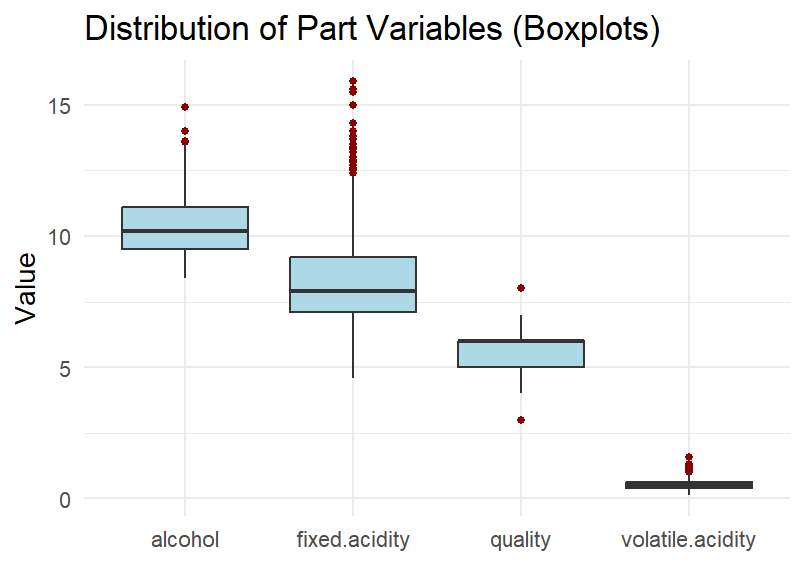
\includegraphics[width=0.5\linewidth]{../plots/bp1} 

}

\caption{Boxplot of part Variables}\label{fig:fig-box}
\end{figure}

\begin{figure}[H]

{\centering 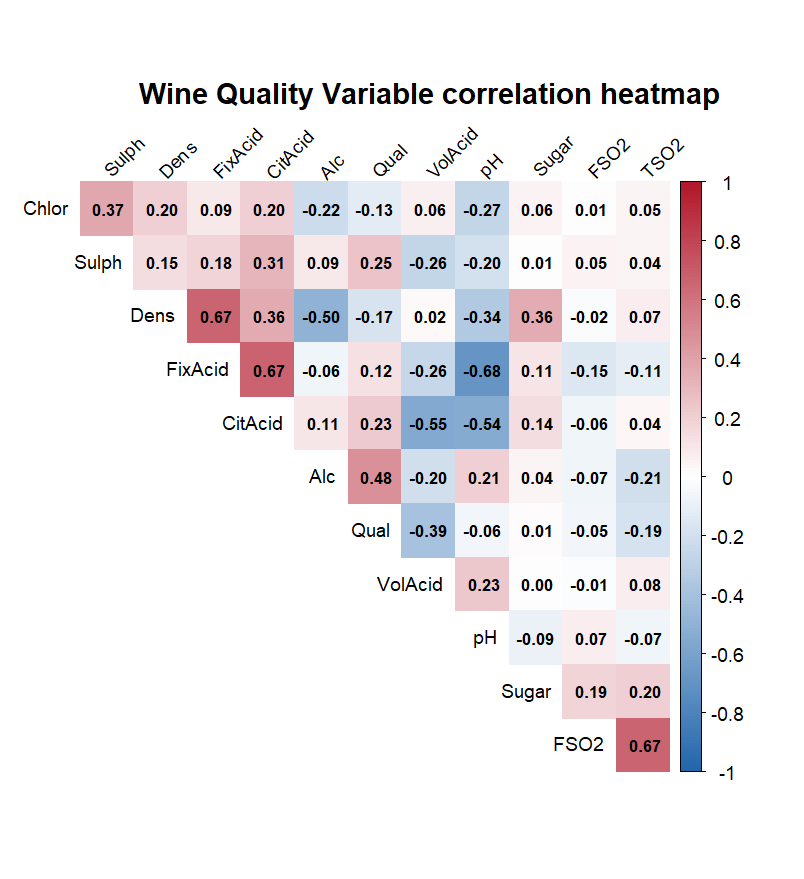
\includegraphics[width=0.5\linewidth]{../plots/r1} 

}

\caption{Heatmap of correlations between variables}\label{fig:heat}
\end{figure}

Figure 2 shows the Pearson correlation coefficient matrix of all eleven variables and the dependent variable wine quality. From the figure, we can see that alcohol and taste show a strong positive correlation (r ≈ +0.48), which indicates that wines with higher alcohol content tend to get higher quality scores. On the other hand, volatile acidity is significantly negatively correlated with health (r ≈ -0.39), indicating that the higher the volatile acidity, the lower the quality score of the wine. We also found that there may be some multicollinearity between the predictors - free SO2 and total SO2 (r = +0.67) and fixed acidity and density (r = +0.67). In short, based on this figure, we have a deeper understanding of the data, and the conclusions we get will help guide the subsequent OLS and Lasso regression methods.

\begin{figure}[H]

{\centering 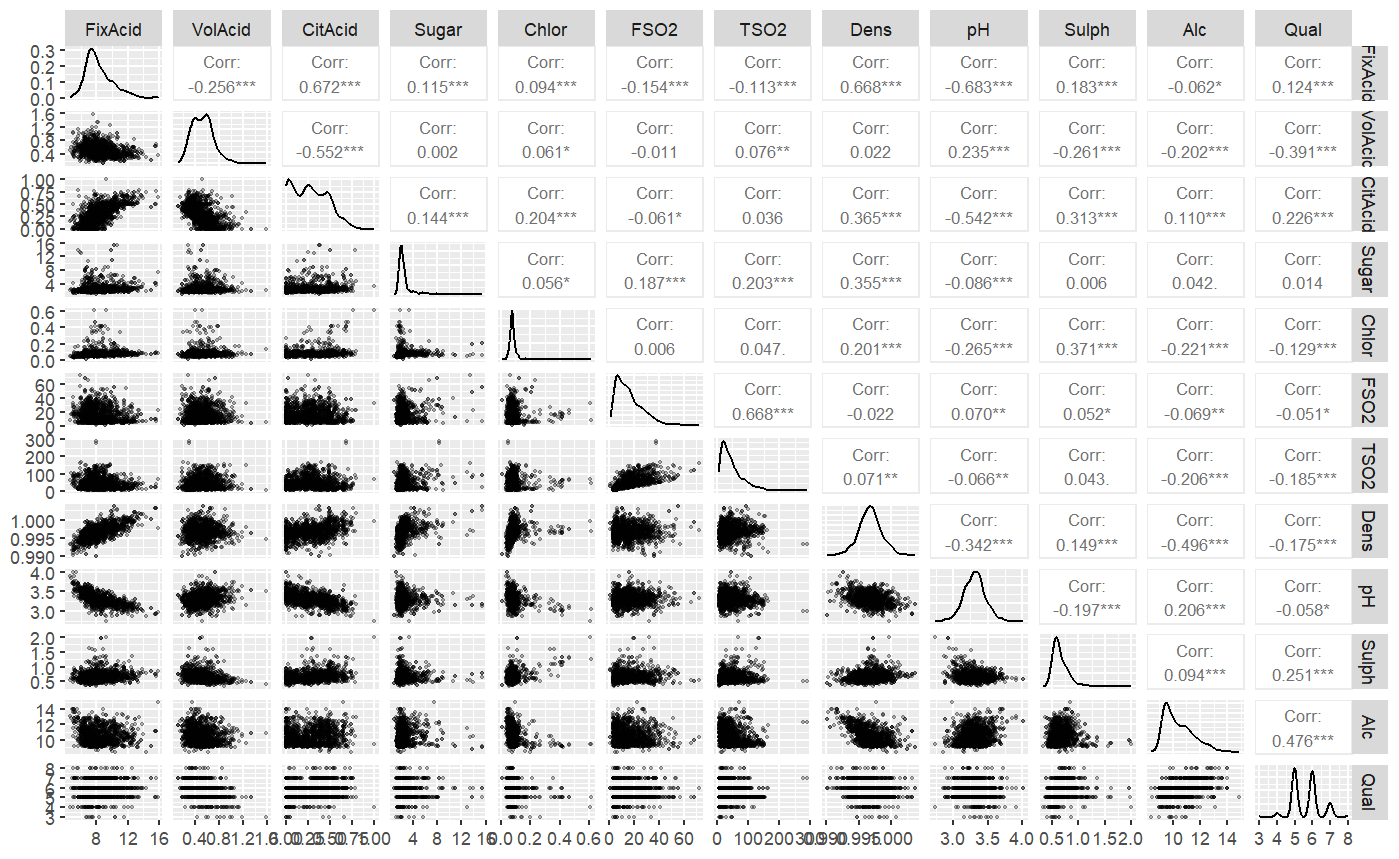
\includegraphics[width=0.5\linewidth]{../plots/p1} 

}

\caption{Pairwise Scatterplot Matrix for all variables}\label{fig:Pairwise}
\end{figure}

Figure 3 uses GGally::ggpairs to output the Pairwise Scatterplot Matrix, where the lower left corner of the diagonal outputs the scatter plots between the variables. From the scatter plots of the variables, we can see that the points of Fixed Acidity and Density are dense and distributed in an upward diagonal, reflecting the conclusion drawn from the heat map that the two variables may be highly collinear. The output in the middle of the diagonal is the kernel density estimates of each variable's marginal distribution, and the output in the upper right corner of the diagonal is the same Pearson correlation coefficient as the heat map. The smooth density curves of each variable reveal the distribution characteristics: for example, Sugar shows an obvious right-skewed long-tail distribution, while Density is highly concentrated in the range of 0.997--0.998. This matrix not only further confirms the known strong associations such as Sulphates and Quality, but also once again shows the multicollinearity problem and the abnormal marginal distribution of some variables, providing a key basis for variable screening and diagnosis of subsequent regression models.

\newpage

\section{4 Methodology \& Results}\label{methodology-results}

\subsection{4.1 Ordinary Least Squares Model (OLS)}\label{ordinary-least-squares-model-ols}

I first used the OLS model to linearly model the dependent variable wine quality for all 11 variables. The regression equation is as follows:
\begin{equation}
\label{eq:ols}
\mathrm{Qual}_i
= \beta_0
+ \beta_1\,\mathrm{FixAcid}_i
+ \beta_2\,\mathrm{VolAcid}_i
+ \cdots
+ \beta_{11}\,\mathrm{Alc}_i
+ \varepsilon_i,
\quad
\varepsilon_i \sim N(0,\sigma^2).
\end{equation}

Hypothesis tests are performed on the parameters to test the significance of the parameters. The results can be obtained from the P-value column in Table 3. For each regression coefficient \(\beta_j\), test:

Null Hypothesis(\(H_0\)) : \(\beta_j\) = 0 vs Alternative Hypothesis(\(H_a\)) : at least one \(\beta_j\) \(≠\) 0

Calculate the \(t\) statistic \(t_j = \hat\beta_j / \mathrm{SE}(\hat\beta_j)\) and report the two-tailed \(p\) value. The results show:

\begin{table}[H]

\begin{center}
\begin{threeparttable}

\caption{\label{tab:ols-model}OLS regression coefficient estimation and significance test}

\begin{tabular}{lllll}
\toprule
 & \multicolumn{1}{c}{Estimate} & \multicolumn{1}{c}{Std. Error} & \multicolumn{1}{c}{t value} & \multicolumn{1}{c}{Pr(>|t|)}\\
\midrule
(Intercept) & 21.97 & 21.19 & 1.04 & 0.30\\
FixAcid & 0.02 & 0.03 & 0.96 & 0.34\\
VolAcid & -1.08 & 0.12 & -8.95 & 0.00\\
CitAcid & -0.18 & 0.15 & -1.24 & 0.21\\
Sugar & 0.02 & 0.02 & 1.09 & 0.28\\
Chlor & -1.87 & 0.42 & -4.47 & 0.00\\
FSO2 & 0.00 & 0.00 & 2.01 & 0.04\\
TSO2 & 0.00 & 0.00 & -4.48 & 0.00\\
Dens & -17.88 & 21.63 & -0.83 & 0.41\\
pH & -0.41 & 0.19 & -2.16 & 0.03\\
Sulph & 0.92 & 0.11 & 8.01 & 0.00\\
Alc & 0.28 & 0.03 & 10.43 & 0.00\\
\bottomrule
\end{tabular}

\end{threeparttable}
\end{center}

\end{table}

Among them, we can find that the parameters of volatile acidity, chloride, total \(SO_2\), free \(SO_2\), pH, sulphates and alcohol are significant in the model, while other variables are not significant at the 5\% level. We can preliminarily conclude that these variables shown as significant above have a certain effect on the quality score of red wine. The fitting results of the OLS model show that the coefficient of determination \(R^2 = 0.3606\) indicates that the model can explain about 36.1\% of the total variance of the quality score. However, after adjustment, \(R^2\) = 0.3561, and the F statistic of the model = 81.35 (df = 11, 1587), \(p<2.2\times10^{-16}\), rejecting the null hypothesis, indicating that the model is significant.

After that, the OLS model residuals were further tested using the diagnosis() function in the library (ds4ling). The following is the output of the OLS residual model diagnostic graph:

\begin{figure}[H]

{\centering 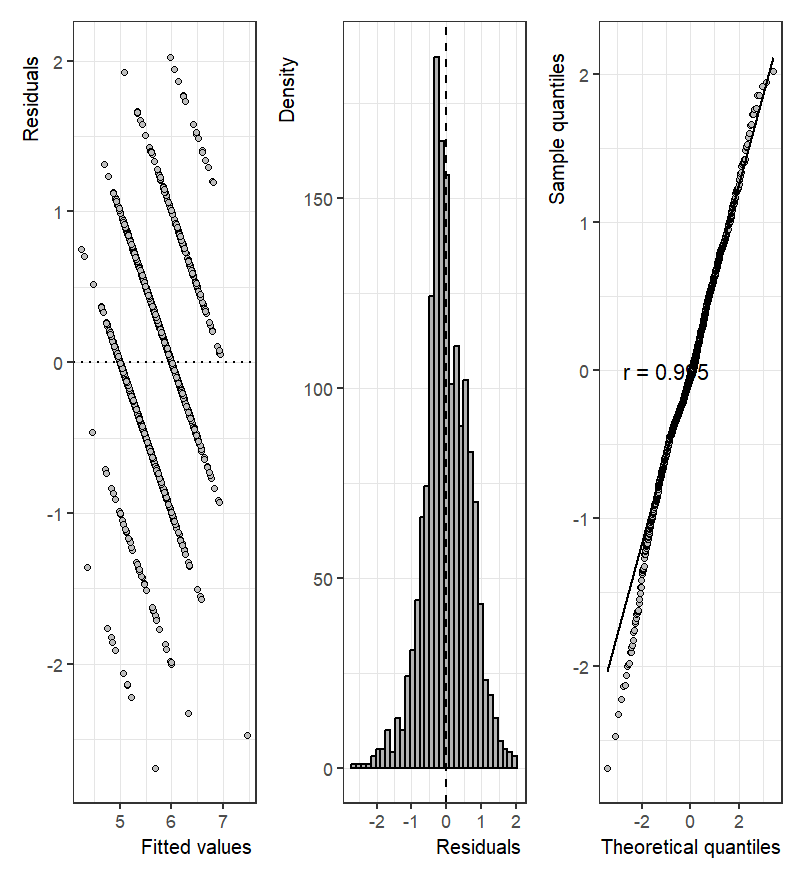
\includegraphics[width=0.5\linewidth]{../plots/OLS_res} 

}

\caption{Residual diagnosis for OLS model}\label{fig:fig-ols-res}
\end{figure}

The residuals vs.~fitted values plot on the left of the test plot shows randomly distributed scatter with no particularly obvious pattern, so the assumption of linearity can be considered supported. However, since the variance seems to increase with the fitted values, there may be slight heteroskedasticity. The Q-Q plot on the right shows that the residuals are roughly distributed along the diagonal (r = 0.95), indicating approximate normality. However, the slight deviation in the tails shows that there may be slight non-normality. The residual density plot in the middle is centered at zero and has a single peak, which is similar to the residual density plot of a good model fit, and is bell-shaped, but a slight skewness is observed.

\subsection{4.2 Lasso Regression}\label{lasso-regression}

To mitigate multicollinearity and enforce sparsity in our predictor set, we fit a Lasso model using the \textbf{glmnet} package. In matrix notation, letting \(x_i\) denote the \(p\)-dimensional predictor vector for observation \(i\) and \(y_i\) its quality score, the Lasso estimate solves

\begin{equation}
\label{eq:lasso}
\min_{\beta_0,\beta}
  \frac{1}{N}\sum_{i=1}^N \bigl(y_i - \beta_0 - x_i^\top \beta\bigr)^2
  \;+\;
  \lambda \sum_{j=1}^p \lvert \beta_j\rvert,
\quad
\lambda \ge 0.
\end{equation}

Prior to fitting, all predictors were standardized and an intercept term retained.
\#\#\# λ Selection via 10-Fold Cross-Validation
Using the glmnet() function, with the penalty parameter \(α\) set to 1, we can get a complete Lasso model. We continue to set the response to the quality of the wine, and the dependent variable is the remaining 11 variables. We hope to use the Lasso model to delete as many unimportant variables as possible, making the model parameters simpler - that is, to get a sparse model. This way, we can more clearly understand which physical and chemical properties (variables) have a more significant impact on the quality of the wine.We then output a plot of \(Log(λ)\) and Mean Square Error to help determine the optimal \(λ\) value.

\begin{figure}[H]

{\centering 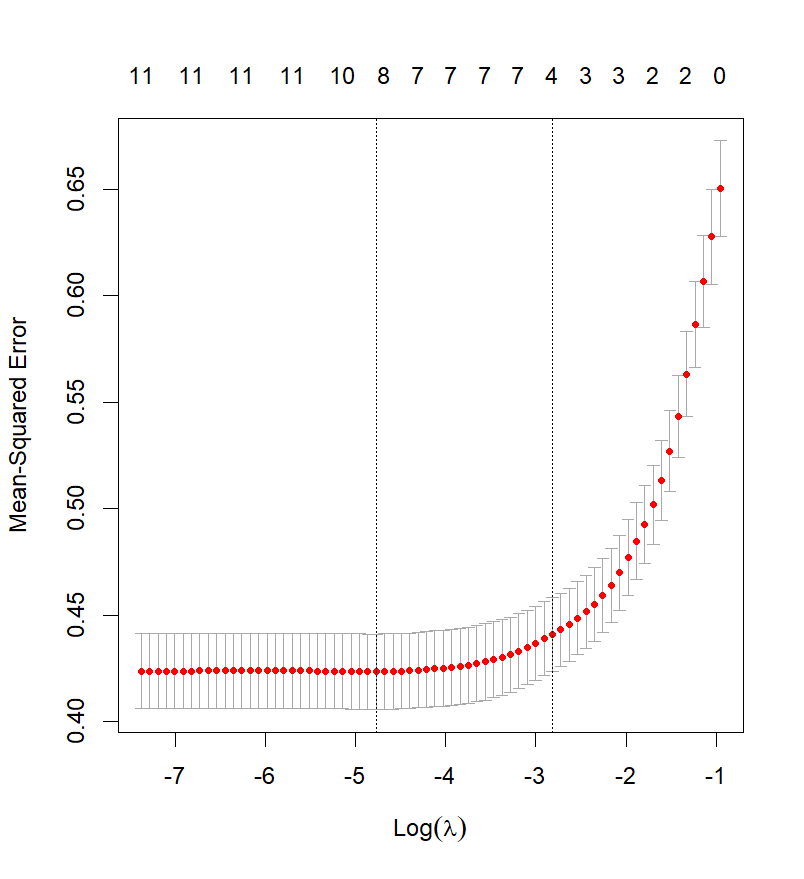
\includegraphics[width=0.5\linewidth]{../plots/cv_lasso} 

}

\caption{Plot of CV\_Lasso}\label{fig:fig-cv-lasso}
\end{figure}

The figure shows that as \(Log(λ)\) increases from -7 to -1, the MSE of the model also increases. To prevent overfitting, we believe that \(Log(λ)\) = -3 is the best value, because reducing \(Log(λ)\) further will penalize the model too much and delete some necessary parameters. The number at the top (11 to 0) indicates the number of factors with non-zero coefficients. As \(λ\) increases, fewer predictors are selected, thereby reducing the complexity of the model. At this optimal \(λ\), Lasso retains the following 8 non-zero coefficients.

Compute the cross-validation MSE for a sequence of \(λ\) values. The value (denoted as \(λ_{min}\)) that minimizes the CV error is found to be.
\(\hatλ_{min}\) = 0.00848

\begin{table}[!h]
\centering
\caption{\label{tab:lasso-coef-table}Non-zero Lasso coefficients at \(\hat{\lambda}_{\min}\)}
\centering
\begin{tabular}[t]{l|l}
\hline
term & estimate\\
\hline
(Intercept) & 4.1628\\
\hline
VolAcid & -1.0243\\
\hline
Sugar & 0.0013\\
\hline
Chlor & -1.7093\\
\hline
FSO2 & 0.0024\\
\hline
TSO2 & -0.0027\\
\hline
pH & -0.3825\\
\hline
Sulph & 0.8196\\
\hline
Alc & 0.2852\\
\hline
\end{tabular}
\end{table}
\newpage

Three predictors:fixed acidity, citric acid, and density are driven exactly to zero, indicating minimal marginal contribution once penalization is applied. The retained coefficients largely mirror OLS signs and magnitudes, reaffirming volatile acidity and chlorides as the negative drivers of quality and sulphates and alcohol content as positive drivers.

Afterwards, I used 10-fold cross validation to compare the prediction performance of OLS and Lasso models.

\begin{figure}[H]

{\centering 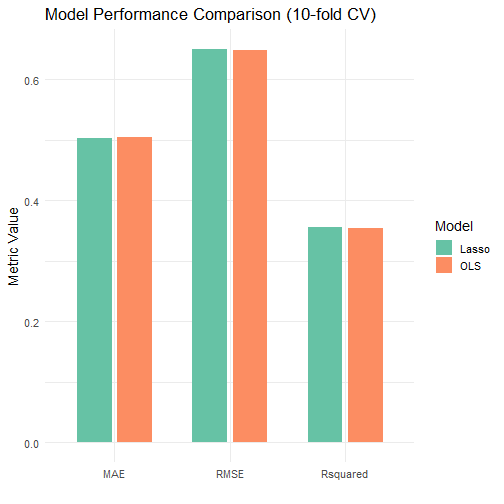
\includegraphics[width=0.5\linewidth]{../plots/cp1} 

}

\caption{OLS and Lasso Model Performance Comparison}\label{fig:figcp}
\end{figure}

From the comparison of the 10-fold cross validation of the two models, it can be seen that LASSO and OLS perform similarly in predicting wine quality, with little difference in MAE, RMSE, and R².

\subsection{5.3 Bayesian Cumulative Logit Regression}\label{bayesian-cumulative-logit-regression}

To account for the ordinal nature of our quality scores (3--8), we replace the Gaussian assumption with a Bayesian cumulative logit model, using the brms package. This framework estimates cutpoints (intercepts) that partition the latent propensity into the seven observed quality levels, and slopes for each predictor, with full posterior uncertainty.
\textbf{Model specification}

\[
\Pr\bigl(\text{Qual}_i \le k \mid x_i\bigr)
=\mathrm{logit}^{-1}\bigl(\gamma_k - x_i^\top\beta\bigr),
\quad k = 1,\dots,7,
\]
where \(\gamma_1<\gamma_2<\cdots<\gamma_7\) are the cutpoints and \(\beta\) the vector of slopes. Priors:

\[
\beta_j \sim \mathrm{Normal}(0,1),\quad 
\gamma_k \sim \mathrm{Normal}(0,5).
\]

The model was fit with four NUTS chains, 2,000 iterations each (1,000 warmup), yielding 4,000 post--warmup draws.

\textbf{Posterior summary \& convergence}\\
Table X reports posterior medians, standard deviations, and 95\% credible intervals for each slope. Convergence diagnostics are excellent (\(\widehat R = 1.00\), Bulk ESS \& Tail ESS \textgreater1,500), though 83 divergent transitions suggest increasing \texttt{adapt\_delta} in future work.

\begin{verbatim}
## Warning: There were 83 divergent transitions after warmup. Increasing
## adapt_delta above 0.8 may help. See
## http://mc-stan.org/misc/warnings.html#divergent-transitions-after-warmup
\end{verbatim}

\begin{table}[!h]
\centering
\caption{(\#tab:tab:bayes-summary)Posterior medians, standard deviations, and 95\% CIs for the Bayesian cumulative logit model}
\centering
\begin{tabular}[t]{l|l|l|l|l}
\hline
Predictor & Median & Est.Error & 2.5% CI & 97.5% CI\\
\hline
Intercept[1] & -4.01 & 2.77 & -9.71 & 1.21\\
\hline
Intercept[2] & -2.29 & 2.40 & -7.02 & 2.25\\
\hline
Intercept[3] & 0.97 & 2.05 & -3.04 & 5.01\\
\hline
Intercept[4] & 2.86 & 2.02 & -1.12 & 6.77\\
\hline
Intercept[5] & 6.52 & 2.02 & 2.57 & 10.44\\
\hline
Intercept[6] & 9.32 & 2.04 & 5.34 & 13.23\\
\hline
Intercept[7] & 12.31 & 2.05 & 8.31 & 16.23\\
\hline
FixAcid & 0.08 & 0.05 & -0.01 & 0.17\\
\hline
VolAcid & -3.17 & 0.36 & -3.88 & -2.46\\
\hline
CitAcid & -0.61 & 0.40 & -1.39 & 0.16\\
\hline
Sugar & 0.04 & 0.04 & -0.04 & 0.12\\
\hline
Chlor & -1.92 & 0.77 & -3.40 & -0.40\\
\hline
FSO2 & 0.02 & 0.01 & 0.00 & 0.03\\
\hline
TSO2 & -0.01 & 0.00 & -0.02 & -0.01\\
\hline
Dens & -0.02 & 1.03 & -2.07 & 1.94\\
\hline
pH & -0.80 & 0.42 & -1.63 & 0.02\\
\hline
Sulph & 2.24 & 0.32 & 1.62 & 2.88\\
\hline
Alc & 0.92 & 0.06 & 0.81 & 1.03\\
\hline
\end{tabular}
\end{table}

Then do the Posterior predictive check for the Bayesian cumulative logit regression model. And use pp\_check() to output the diagnosis figure:

\begin{figure}[H]

{\centering 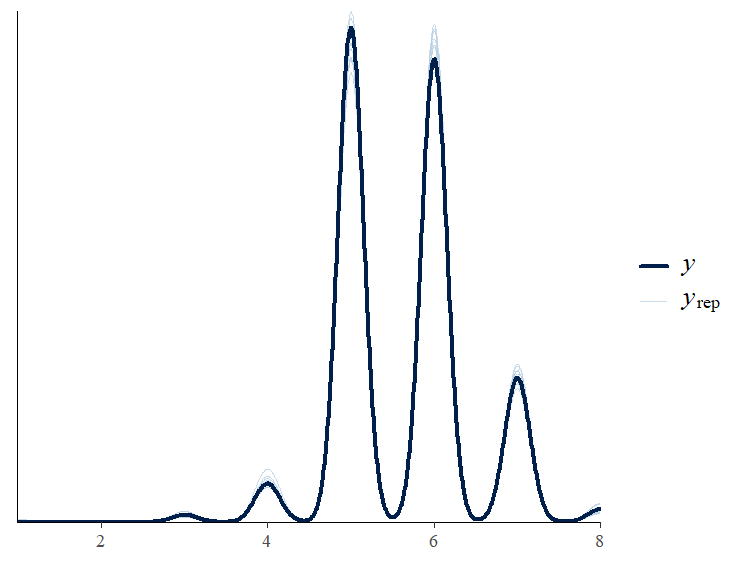
\includegraphics[width=0.6\linewidth]{../plots/kde} 

}

\caption{Posterior predictive check: observed vs. replicated quality distributions}\label{fig:ppck}
\end{figure}

Figure 7 overlays the kernel density of the observed quality distribution (\(y\), dark blue) against 10 replicated datasets (\(y_{rep}\), light blue). The replicated densities closely track the empirical peaks at scores 5, 6 and 7, demonstrating that the model captures the overall shape and modal structure of the data, with only extreme slight under‐coverage of the low (3--4) tail and large(7-8) tail.

\section{6 Conclusion and Future Directions}\label{conclusion-and-future-directions}

\subsection{}\label{section}

\subsection{Participants}\label{participants}

\subsection{Material}\label{material}

\subsection{Procedure}\label{procedure}

\subsection{Data analysis}\label{data-analysis}

We used R (Version 4.4.2; R Core Team, 2024) and the R-packages \emph{papaja} (Version 0.1.3; Aust \& Barth, 2024) and \emph{tinylabels} (Version 0.2.5; Barth, 2025) for all our analyses.

\section{Results}\label{results}

\section{Discussion}\label{discussion}

\newpage

\section{References}\label{references}

\phantomsection\label{refs}
\begin{CSLReferences}{1}{0}
\bibitem[\citeproctext]{ref-R-papaja}
Aust, F., \& Barth, M. (2024). \emph{{papaja}: {Prepare} reproducible {APA} journal articles with {R Markdown}}. \url{https://doi.org/10.32614/CRAN.package.papaja}

\bibitem[\citeproctext]{ref-R-tinylabels}
Barth, M. (2025). \emph{{tinylabels}: Lightweight variable labels}. \url{https://doi.org/10.32614/CRAN.package.tinylabels}

\bibitem[\citeproctext]{ref-R-base}
R Core Team. (2024). \emph{R: A language and environment for statistical computing}. Vienna, Austria: R Foundation for Statistical Computing. Retrieved from \url{https://www.R-project.org/}

\end{CSLReferences}


\end{document}
